% Created 2021-08-13 Fri 16:22
% Intended LaTeX compiler: pdflatex
\documentclass[11pt]{article}
\usepackage[utf8]{inputenc}
\usepackage[T1]{fontenc}
\usepackage{graphicx}
\usepackage{grffile}
\usepackage{longtable}
\usepackage{wrapfig}
\usepackage{rotating}
\usepackage[normalem]{ulem}
\usepackage{amsmath}
\usepackage{textcomp}
\usepackage{amssymb}
\usepackage{capt-of}
\usepackage{hyperref}
\author{Sreejith Sreekumar}
\date{\today}
\title{Engineering New Features}
\hypersetup{
 pdfauthor={Sreejith Sreekumar},
 pdftitle={Engineering New Features},
 pdfkeywords={},
 pdfsubject={},
 pdfcreator={Emacs 26.3 (Org mode 9.1.9)}, 
 pdflang={English}}
\begin{document}

\maketitle
\tableofcontents

\begin{itemize}
\item Linear models cannot include variable interations. This forces us to add variable interations explicitly
\item Models like RF, GB Trees, NNs do not require this
\end{itemize}

\section{Using volume (Number of stocks traded per day) as one of the features}
\label{sec:orgdd39f29}

\begin{verbatim}

# Create 2 new volume features, 1-day % change and 5-day SMA of the % change
new_features = ['Adj_Volume_1d_change', 'Adj_Volume_1d_change_SMA']
feature_names.extend(new_features)
lng_df["Adj_Volume_1d_change"] = lng_df['Adj_Volume'].pct_change()
lng_df["Adj_Volume_1d_change_SMA"] = talib.SMA(lng_df["Adj_Volume_1d_change"].values,
                        timeperiod=5)

# Plot histogram of volume % change data
lng_df[new_features].plot(kind='hist', sharex=False, bins=50)
plt.show()


\end{verbatim}

\begin{center}
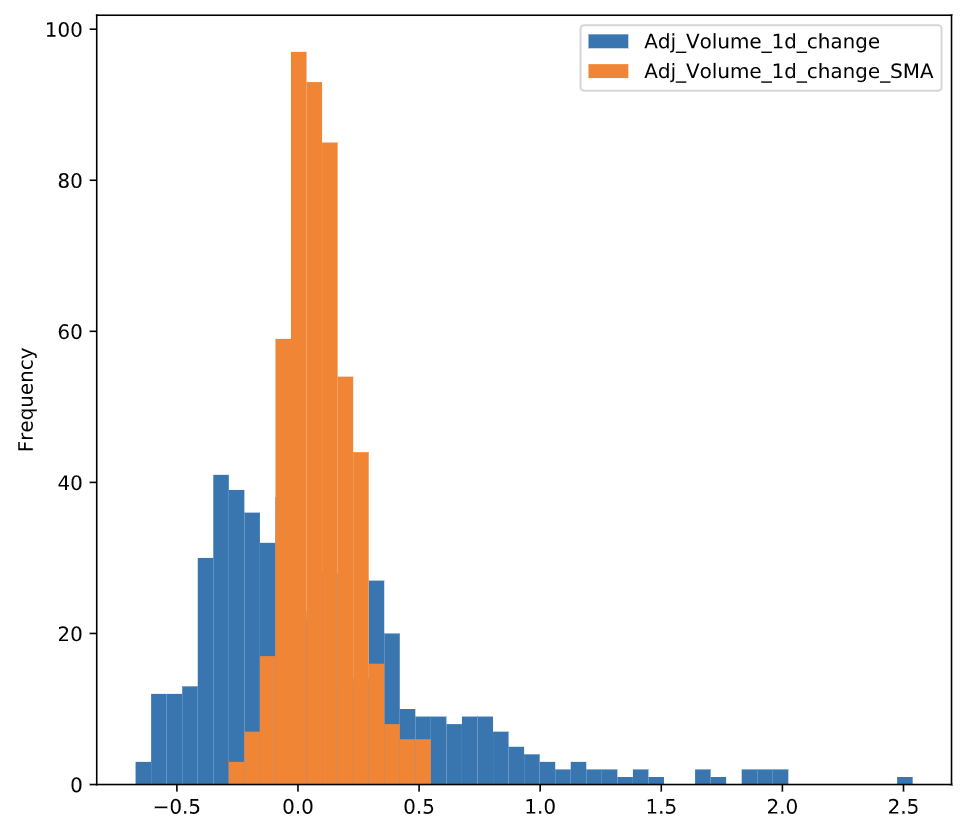
\includegraphics[width=.9\linewidth]{new-features.png}
\end{center}


\section{Weekdays as Features}
\label{sec:orgd5b926c}

\begin{verbatim}
# Add the weekday labels to the new_features list
new_features.extend(["weekday_" + str(i) for i in range(1, 5)])

# Plot the correlations between the new features and the targets
sns.heatmap(lng_df[new_features + ['5d_close_future_pct']].corr(), annot=True)
plt.yticks(rotation=0)  # ensure y-axis ticklabels are horizontal
plt.xticks(rotation=90)  # ensure x-axis ticklabels are vertical
plt.tight_layout()
plt.show()
\end{verbatim}


\begin{center}
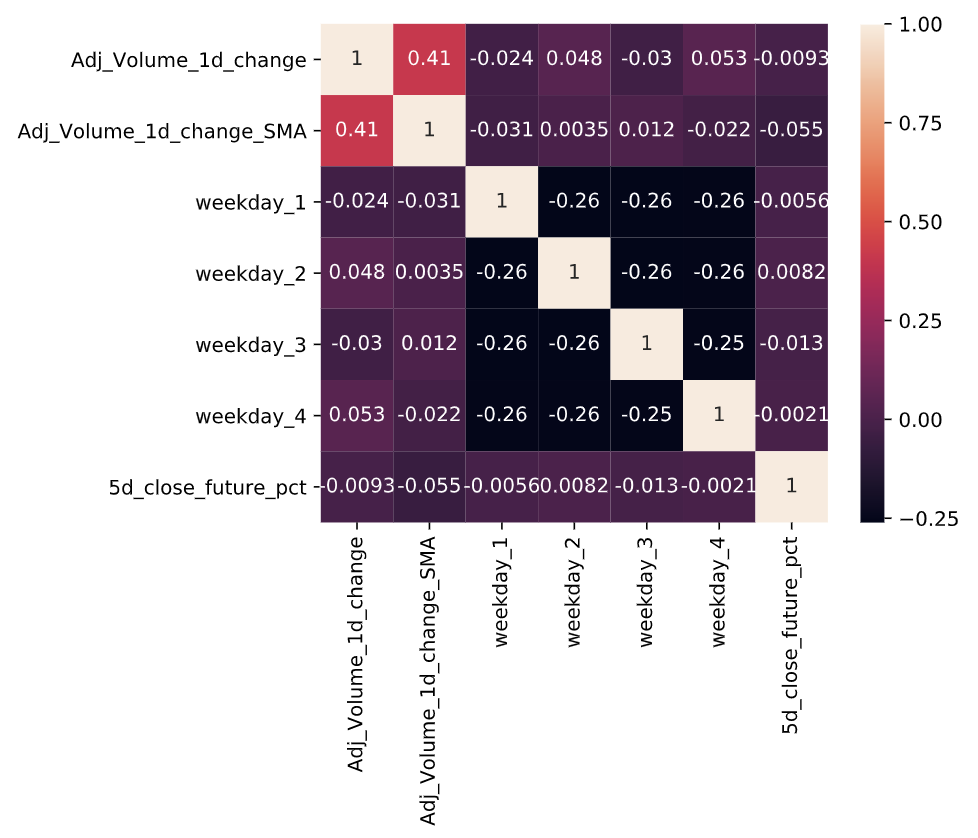
\includegraphics[width=.9\linewidth]{weekday-corr.png}
\end{center}
\end{document}